% Options for packages loaded elsewhere
\PassOptionsToPackage{unicode}{hyperref}
\PassOptionsToPackage{hyphens}{url}
\PassOptionsToPackage{dvipsnames,svgnames,x11names}{xcolor}
%
\documentclass[
  letterpaper,
  11pt,
  english,
  doublespacing,
  headsepline,
  consistentlayout,
  oneside,
  openany]{MastersDoctoralThesis}

\usepackage{amsmath,amssymb}
\usepackage{iftex}
\ifPDFTeX
  \usepackage[T1]{fontenc}
  \usepackage[utf8]{inputenc}
  \usepackage{textcomp} % provide euro and other symbols
\else % if luatex or xetex
  \usepackage{unicode-math}
  \defaultfontfeatures{Scale=MatchLowercase}
  \defaultfontfeatures[\rmfamily]{Ligatures=TeX,Scale=1}
\fi
\usepackage{lmodern}
\ifPDFTeX\else  
    % xetex/luatex font selection
\fi
% Use upquote if available, for straight quotes in verbatim environments
\IfFileExists{upquote.sty}{\usepackage{upquote}}{}
\IfFileExists{microtype.sty}{% use microtype if available
  \usepackage[]{microtype}
  \UseMicrotypeSet[protrusion]{basicmath} % disable protrusion for tt fonts
}{}
\usepackage{xcolor}
\usepackage[paper=a4paper,inner=3.0cm,outer=2.0cm,bindingoffset=0cm,top=1.5cm,bottom=1.5cm]{geometry}
\setlength{\emergencystretch}{3em} % prevent overfull lines
\setcounter{secnumdepth}{5}
% Make \paragraph and \subparagraph free-standing
\makeatletter
\ifx\paragraph\undefined\else
  \let\oldparagraph\paragraph
  \renewcommand{\paragraph}{
    \@ifstar
      \xxxParagraphStar
      \xxxParagraphNoStar
  }
  \newcommand{\xxxParagraphStar}[1]{\oldparagraph*{#1}\mbox{}}
  \newcommand{\xxxParagraphNoStar}[1]{\oldparagraph{#1}\mbox{}}
\fi
\ifx\subparagraph\undefined\else
  \let\oldsubparagraph\subparagraph
  \renewcommand{\subparagraph}{
    \@ifstar
      \xxxSubParagraphStar
      \xxxSubParagraphNoStar
  }
  \newcommand{\xxxSubParagraphStar}[1]{\oldsubparagraph*{#1}\mbox{}}
  \newcommand{\xxxSubParagraphNoStar}[1]{\oldsubparagraph{#1}\mbox{}}
\fi
\makeatother


\providecommand{\tightlist}{%
  \setlength{\itemsep}{0pt}\setlength{\parskip}{0pt}}\usepackage{longtable,booktabs,array}
\usepackage{calc} % for calculating minipage widths
% Correct order of tables after \paragraph or \subparagraph
\usepackage{etoolbox}
\makeatletter
\patchcmd\longtable{\par}{\if@noskipsec\mbox{}\fi\par}{}{}
\makeatother
% Allow footnotes in longtable head/foot
\IfFileExists{footnotehyper.sty}{\usepackage{footnotehyper}}{\usepackage{footnote}}
\makesavenoteenv{longtable}
\usepackage{graphicx}
\makeatletter
\def\maxwidth{\ifdim\Gin@nat@width>\linewidth\linewidth\else\Gin@nat@width\fi}
\def\maxheight{\ifdim\Gin@nat@height>\textheight\textheight\else\Gin@nat@height\fi}
\makeatother
% Scale images if necessary, so that they will not overflow the page
% margins by default, and it is still possible to overwrite the defaults
% using explicit options in \includegraphics[width, height, ...]{}
\setkeys{Gin}{width=\maxwidth,height=\maxheight,keepaspectratio}
% Set default figure placement to htbp
\makeatletter
\def\fps@figure{htbp}
\makeatother
% definitions for citeproc citations
\NewDocumentCommand\citeproctext{}{}
\NewDocumentCommand\citeproc{mm}{%
  \begingroup\def\citeproctext{#2}\cite{#1}\endgroup}
\makeatletter
 % allow citations to break across lines
 \let\@cite@ofmt\@firstofone
 % avoid brackets around text for \cite:
 \def\@biblabel#1{}
 \def\@cite#1#2{{#1\if@tempswa , #2\fi}}
\makeatother
\newlength{\cslhangindent}
\setlength{\cslhangindent}{1.5em}
\newlength{\csllabelwidth}
\setlength{\csllabelwidth}{3em}
\newenvironment{CSLReferences}[2] % #1 hanging-indent, #2 entry-spacing
 {\begin{list}{}{%
  \setlength{\itemindent}{0pt}
  \setlength{\leftmargin}{0pt}
  \setlength{\parsep}{0pt}
  % turn on hanging indent if param 1 is 1
  \ifodd #1
   \setlength{\leftmargin}{\cslhangindent}
   \setlength{\itemindent}{-1\cslhangindent}
  \fi
  % set entry spacing
  \setlength{\itemsep}{#2\baselineskip}}}
 {\end{list}}
\usepackage{calc}
\newcommand{\CSLBlock}[1]{\hfill\break\parbox[t]{\linewidth}{\strut\ignorespaces#1\strut}}
\newcommand{\CSLLeftMargin}[1]{\parbox[t]{\csllabelwidth}{\strut#1\strut}}
\newcommand{\CSLRightInline}[1]{\parbox[t]{\linewidth - \csllabelwidth}{\strut#1\strut}}
\newcommand{\CSLIndent}[1]{\hspace{\cslhangindent}#1}

\usepackage{etoolbox}
\usepackage{setspace}

% Ajustamos el entorno CSLReferences (que Pandoc/Quarto usa para las referencias):
\AtBeginEnvironment{CSLReferences}{
    \singlespacing          % o " \onehalfspacing " si quieres algo intermedio
    \setlength{\parskip}{0pt}     % o un valor peque�o (ej. 2pt) si deseas m�s separaci�n entre p�rrafos
    \setlength{\itemsep}{0.25em}  % reduce el espacio entre �tems (ajusta seg�n tu preferencia)
}
%\usepackage[utf8]{inputenc} % Required for inputting international characters
%\usepackage[T1]{fontenc} % Output font encoding for international characters; causes problems for xelatex

%\usepackage{mathpazo} % Use the Palatino font by default

%\usepackage[backend=bibtex, style=authoryear, natbib=true]{biblatex} % Use the bibtex backend with the authoryear citation style (which resembles APA)

\usepackage[autostyle=true]{csquotes} % Required to generate language-dependent quotes in the bibliography

\usepackage{pdfpages}
\usepackage{etoolbox} % para la tabla de contenido y figura y tablas

% Paquetes adicionales que no están en MastersDoctoralThesis.cls
\usepackage{bbm}  % Bold math symbols
\usepackage{mathrsfs}  % Script math fonts
%\usepackage{siunitx}  % Scientific notation (verificar si ya está en cls)
\usepackage{url}  % URLs
\usepackage{color}  % Color support
\usepackage{mathtools}  % Extended math tools
%\usepackage{float}  % Better float control
\usepackage{array}  % Advanced table formatting
\usepackage{multirow}  % Table multirows
\usepackage{wrapfig}  % Wrapping text around figures
\usepackage{colortbl}  % Table colors
\usepackage{pdflscape}  % Landscape pages
\usepackage{xcolor}  % Advanced colors
%\usepackage{amsmath}  % Math symbols

\usepackage{float}

%\usepackage{amsfonts}
%\usepackage{amssymb}

% Re-ajustar el setup sólo para las figuras
% \captionsetup[figure]{position=above}
% \floatstyle{plaintop}
% \restylefloat{figure}

% \usepackage{etoolbox}
% 
% % Para TODAS las figuras
% \AtEndEnvironment{figure}{
%   \par\medskip
%   \centering
%   \small Source: Author
% }
% 
% % Para TODAS las tablas
% \AtEndEnvironment{table}{
%   \par\medskip
%   \centering
%   \small Source: Author
% }

%----------------------------------------------------------------------------------------
%	MARGINS
%----------------------------------------------------------------------------------------

\geometry{
	headheight=4ex,
	includehead,
	includefoot
}

\raggedbottom

\AtBeginDocument{
\hypersetup{pdftitle=\ttitle} % Set the PDF's title to your title
\hypersetup{pdfauthor=\authorname} % Set the PDF's author to your name
\hypersetup{pdfkeywords=\keywordnames} % Set the PDF's keywords to your keywords
}

%---------------------------------------------
\usepackage{booktabs}
\usepackage{longtable}
\usepackage{array}
\usepackage{multirow}
\usepackage{wrapfig}
\usepackage{float}
\usepackage{colortbl}
\usepackage{pdflscape}
\usepackage{tabu}
\usepackage{threeparttable}
\usepackage{threeparttablex}
\usepackage[normalem]{ulem}
\usepackage{makecell}
\usepackage{xcolor}
\setlength{\parindent}{15pt}
\setlength{\parskip}{0pt}
\makeatletter
\@ifpackageloaded{bookmark}{}{\usepackage{bookmark}}
\makeatother
\makeatletter
\@ifpackageloaded{caption}{}{\usepackage{caption}}
\AtBeginDocument{%
\ifdefined\contentsname
  \renewcommand*\contentsname{Table of contents}
\else
  \newcommand\contentsname{Table of contents}
\fi
\ifdefined\listfigurename
  \renewcommand*\listfigurename{List of Figures}
\else
  \newcommand\listfigurename{List of Figures}
\fi
\ifdefined\listtablename
  \renewcommand*\listtablename{List of Tables}
\else
  \newcommand\listtablename{List of Tables}
\fi
\ifdefined\figurename
  \renewcommand*\figurename{Figure}
\else
  \newcommand\figurename{Figure}
\fi
\ifdefined\tablename
  \renewcommand*\tablename{Table}
\else
  \newcommand\tablename{Table}
\fi
}
\@ifpackageloaded{float}{}{\usepackage{float}}
\floatstyle{ruled}
\@ifundefined{c@chapter}{\newfloat{codelisting}{h}{lop}}{\newfloat{codelisting}{h}{lop}[chapter]}
\floatname{codelisting}{Listing}
\newcommand*\listoflistings{\listof{codelisting}{List of Listings}}
\makeatother
\makeatletter
\makeatother
\makeatletter
\@ifpackageloaded{caption}{}{\usepackage{caption}}
\@ifpackageloaded{subcaption}{}{\usepackage{subcaption}}
\makeatother
\ifLuaTeX
  \usepackage{selnolig}  % disable illegal ligatures
\fi
\usepackage{bookmark}

\IfFileExists{xurl.sty}{\usepackage{xurl}}{} % add URL line breaks if available
\urlstyle{same} % disable monospaced font for URLs
\hypersetup{
  pdftitle={A doctoral thesis},
  pdfauthor={Jane Doe},
  colorlinks=true,
  linkcolor={blue},
  filecolor={Maroon},
  citecolor={black},
  urlcolor={black},
  pdfcreator={LaTeX via pandoc}}

\thesistitle{A doctoral
thesis} % Your thesis title, this is used in the title and abstract, print it elsewhere with \ttitle
\supervisor{Dr.~Ashok
Kunil} % Your supervisor's name, this is used in the title page, print it elsewhere with \supname
\examiner{} % Your examiner's name, this is not currently used anywhere in the template, print it elsewhere with \examname
\degree{Doctor of
Philosophy} % Your degree name, this is used in the title page and abstract, print it elsewhere with \degreename
\author{Jane
Doe} % Your name, this is used in the title page and abstract, print it elsewhere with \authorname
\addresses{} % Your address, this is not currently used anywhere in the template, print it elsewhere with \addressname

\subject{} % Your subject area, this is not currently used anywhere in the template, print it elsewhere with \subjectname
\keywords{} % Keywords for your thesis, this is not currently used anywhere in the template, print it elsewhere with \keywordnames
\university{University of
Ottawa} % Your university's name, this is used in the title page and abstract, print it elsewhere with \univname
\department{Department of
Mathematics} % Your department's name, this is used in the title page and abstract, print it elsewhere with \deptname
\group{Informatics
Program} % Your research group's name and URL, this is used in the title page, print it elsewhere with \groupname
\faculty{Applied Math
Group} % Your faculty's name and URL, this is used in the title page and abstract, print it elsewhere with \facname

\setcounter{tocdepth}{2} % The depth to which the document sections are printed to the table of contents
\begin{document}
 \makeatletter
\renewcommand{\cleardoublepage}{\clearpage} % Evita páginas en blanco extra
\makeatother

\frontmatter % Use roman page numbering style (i, ii, iii, iv...) for the pre-content pages

\pagestyle{plain} % Default to the plain heading style until the thesis style is called for the body content

%----------------------------------------------------------------------------------------
%	TITLE PAGE
%----------------------------------------------------------------------------------------


\begin{titlepage}
  \begin{center}
  
    % LOGO ARRIBA
    % Ajusta la ruta y el tamaño de tu logo (o quítalo si no quieres poner imagen)
									
\includegraphics[height=3.5cm]{images/ufpe-logo.png} % University/department logo
						\\[0.3cm]
    %
\includegraphics[width=2cm]{images/ufpe-logo.png}\\[0.3cm]
    
    % NOMBRES DE LA UNIVERSIDAD/PROGRAMA EN MAYÚSCULAS
    {\large\MakeUppercase{UNIVERSIDADE FEDERAL DE PERNAMBUCO}}\\
    {\large\MakeUppercase{CENTRO DE CIÊNCIAS EXATAS E DA NATUREZA}}\\
    {\large\MakeUppercase{PROGRAMA DE PÓS-GRADUAÇÃO EM ESTATÍSTICA}}\\
    {\large\MakeUppercase{DOUTORADO EM ESTATÍSTICA}}\\[4cm]
		
    % NOMBRE DE LA TESISTA
    {\large ROSA JANETH ALPALA}\\[3cm]
    
    % TÍTULO 
    {\Large \textbf{TEST STATISTICS BASED ON ENTROPY FOR HETEROGENEITY DETECTION IN SAR DATA}}\\[6cm]
    %\textbf{AND CAUSE-SPECIFIC MORTALITY IN ENGLAND}}\\[5cm]
    

		
		%{\Large Doctoral Thesis}\\[2cm] % Thesis type
%
    % CIUDAD Y AÑO
   {\large Recife}\\
   {\large 2025}
    
  \end{center}
\end{titlepage}

\begin{titlepage}
  \thispagestyle{empty}
    \begin{center}
    {\large ROSA JANETH ALPALA}\\[4cm]
    {\Large \textbf{TEST STATISTICS BASED ON ENTROPY FOR HETEROGENEITY 
    DETECTION IN SAR DATA }}\\[4cm]
  \end{center}

  % Quita el \hfill y en lugar de eso usamos \begin{center}...
  %\begin{center}
  \noindent
  \hspace*{0.3\textwidth}
  \begin{minipage}{0.65\textwidth}
    Thesis submitted to the Graduate Program in Statistics of 
    the Universidade Federal de Pernambuco, as a partial requirement 
    for the degree of Doctor of Philosophy  in Statistics.
    
    \vspace{1em}
    \textbf{Concentration area}: Applied Statistics
    
    \vspace{2em} 
    \textbf{Advisor}: Prof. Alejandro C. Frery \\
    \textbf{Co-advisor}: Prof. Abraão David Costa do Nascimento
  \end{minipage}
  %\end{center}
  
  \vfill
  \begin{center}
    Recife\\
    2025
  \end{center}
\end{titlepage}

% --- SUBPORTADA O FOLHA DE ROSTO ---

% \begin{titlepage}
%   \thispagestyle{empty} % Quita numeración en esta página
%   
%   \begin{center}
%     % --- NOMBRE DEL ESTUDIANTE --- 
%     {\large ROSA JANETH ALPALA}\\[3cm]
%     
%     % --- TÍTULO EN MAYÚSCULAS O NEGRITA --- 
%     {\Large \textbf{TEST STATISTICS BASED ON ENTROPY FOR HETEROGENEITY DETECTION IN SAR DATA }}\\[3cm]
%     %\textbf{}}\\[3cm]
%   \end{center}
% %Test Statistics Based on Entropy and the Coefficient of Variation for Heterogeneity Detection in SAR Data
%   \hfill
%   \begin{minipage}{0.6\textwidth}
%     % -- TEXTO DESCRIPTIVO --
%     Thesis submitted to the Graduate Program in Statistics of the Universidade Federal de Pernambuco, as a partial requirement for the degree of Doctor in Statistics.
%     
%     \vspace{1em}
%     \textbf{Concentration area}: Applied Statistics
%     
%     \vspace{2em} 
% 		\textbf{Advisor}: Prof. Alejandro C. Frery \\
% 		\textbf{Co-advisor}: Prof. Abraão David Costa do Nascimento
%    
%   \end{minipage}
%   
%   \vfill
%   \begin{center}
%     Recife\\
%     2025
%   \end{center}
% 
% \end{titlepage}

%----------------------------------------------------------------------------------------
%	Actas
%----------------------------------------------------------------------------------------
%\cleardoublepage % Asegura que la portada termine en una página aparte
%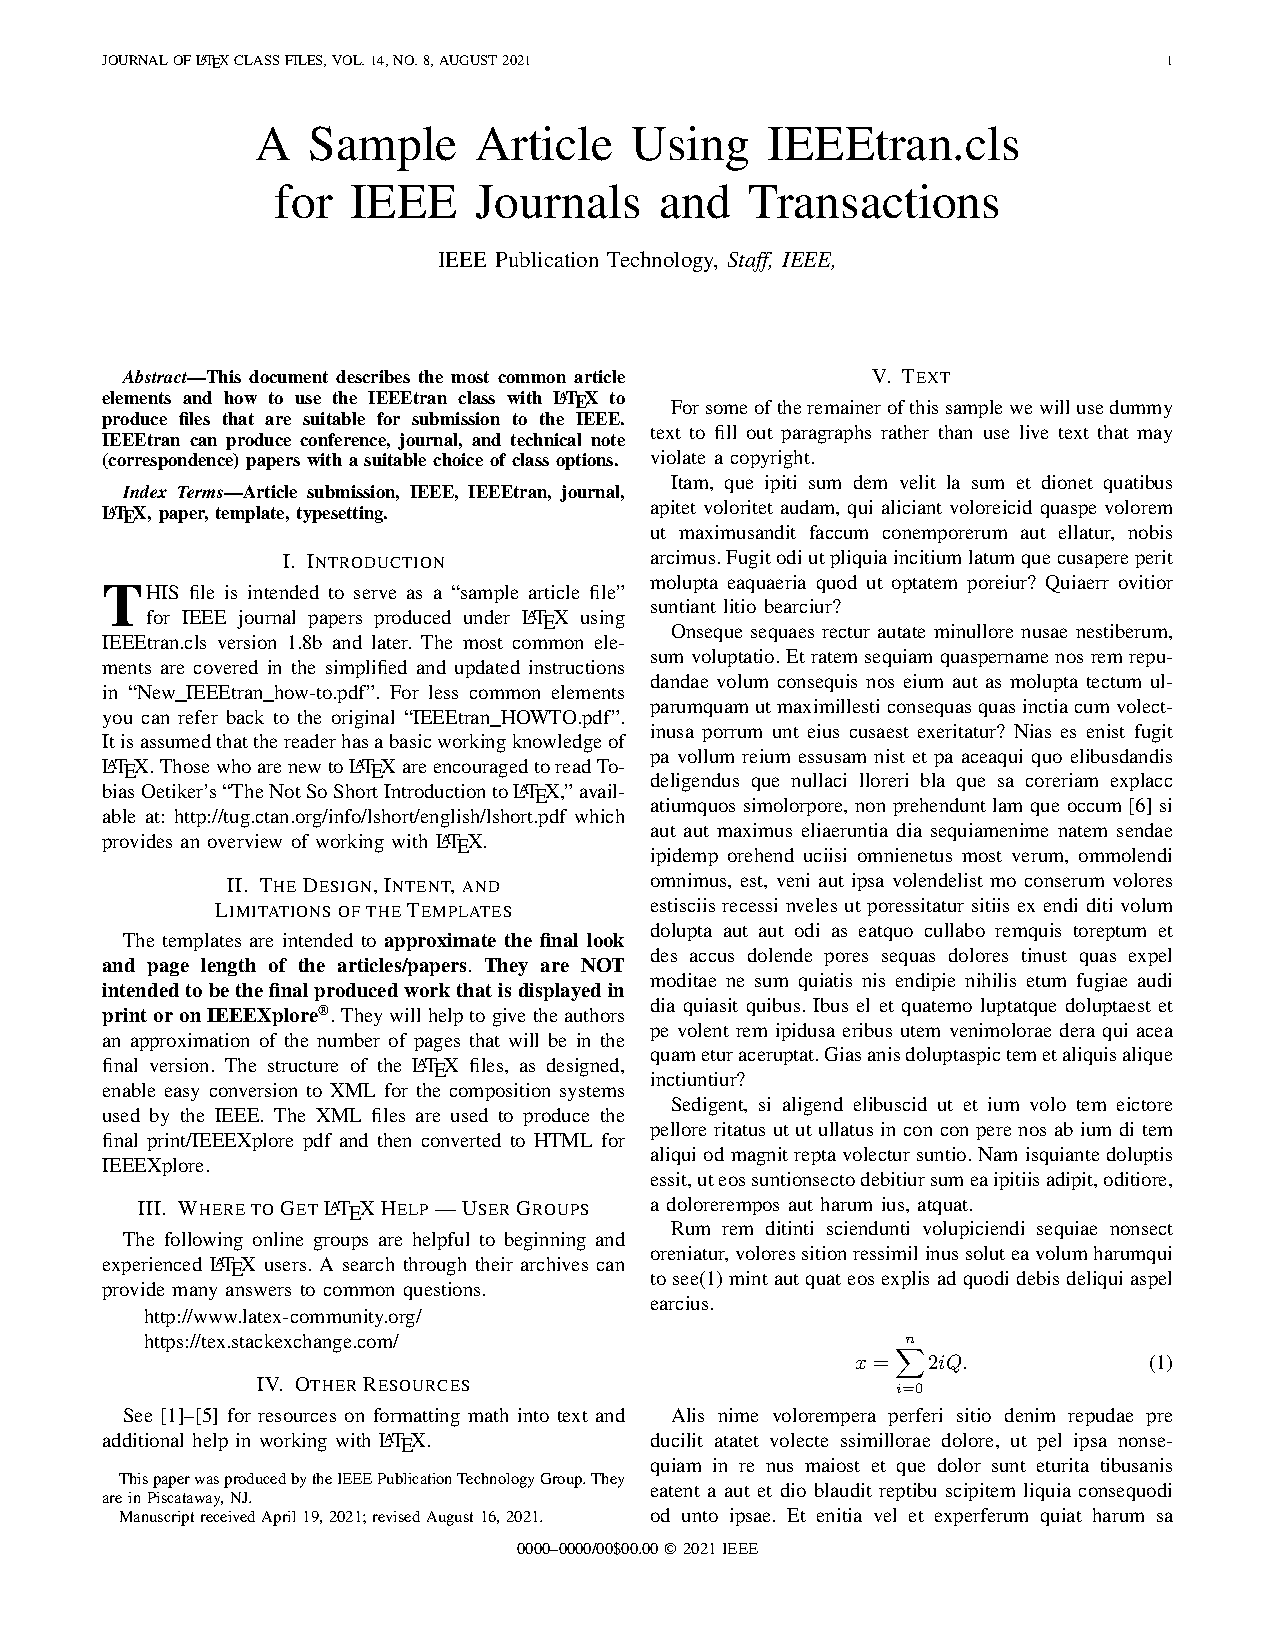
\includepdf[pages=-]{Frontmatter/acta.pdf}
%\cleardoublepage



%----------------------------------------------------------------------------------------
%	ACKNOWLEDGEMENTS
%----------------------------------------------------------------------------------------

%\begin{acknowledgements}
%%\addchaptertocentry{\acknowledgementname} % Add the acknowledgements to the table of contents
%%\begin{acknowledgements}
\addchaptertocentry{\acknowledgementname} % Add the acknowledgements to the table of contents
This PhD project is the outcome of the work of many people: 
\\
Whenever fitting, specific acknowledgements are given inside the text or in footnotes, but here I would especially like to thank all of my colleagues at \\
In particular, 



%\newpage
%\section*{Author's note}
%This thesis has been compressed for uploading and is missing hyperlinks.
%The original version, containing full-resolution images and hyperlinks, can be obtained from \url{http://users.ictp.it/~afantini/PhD_thesis/PhD_thesis_final_15feb2019.pdf} or by requesting it to \href{mailto:adr.fantini@gmail.com}{adr.fantini@gmail.com}.


\end{acknowledgements}
%%\end{acknowledgements}
%
% 

\begingroup
\renewcommand{\abovechapterskip}{\vspace*{15pt}}  % En lugar de 20pt
  \renewcommand{\chapterbelowskip}{\vspace*{20pt}}  % En lugar de 40pt
  % Aquí redefinimos las macros solo para este entorno
  \renewcommand{\chapteralign}{\centering}      % Centra el título
  \renewcommand{\chapterfont}{\bfseries\Large}  % Negrita y tamaño grande (ajusta a gusto)

  \begin{acknowledgements}
  %\addchaptertocentry{\acknowledgementname} % Add the acknowledgements to the table of contents
  
    \begin{acknowledgements}
\addchaptertocentry{\acknowledgementname} % Add the acknowledgements to the table of contents
This PhD project is the outcome of the work of many people: 
\\
Whenever fitting, specific acknowledgements are given inside the text or in footnotes, but here I would especially like to thank all of my colleagues at \\
In particular, 



%\newpage
%\section*{Author's note}
%This thesis has been compressed for uploading and is missing hyperlinks.
%The original version, containing full-resolution images and hyperlinks, can be obtained from \url{http://users.ictp.it/~afantini/PhD_thesis/PhD_thesis_final_15feb2019.pdf} or by requesting it to \href{mailto:adr.fantini@gmail.com}{adr.fantini@gmail.com}.


\end{acknowledgements}
  
  \end{acknowledgements}
\endgroup

%%----------------------------------------------------------------------------------------
%%	DECLARATION PAGE
%%----------------------------------------------------------------------------------------
%%
%
%

\begingroup
\renewcommand{\abovechapterskip}{\vspace*{10pt}}  % En lugar de 20pt
  \renewcommand{\chapterbelowskip}{\vspace*{10pt}}  % En lugar de 40pt
  % Aquí redefinimos las macros solo para este entorno
  \renewcommand{\chapteralign}{\centering}      % Centra el título
  \renewcommand{\chapterfont}{\bfseries\Large}  % Negrita y tamaño grande (ajusta a gusto)
\begin{abstract}
%\begin{otherlanguage}{spanish}
%\begin{abstract}
%\phantomsection
%\addcontentsline{toc}{chapter}{Abstract}

This work  presents a statistical approach to detect heterogeneity 
in synthetic aperture radar (SAR) intensity data using entropy-based methods.
In homogeneous regions, where fully developed speckle is present, SAR returns 
are well modeled by the Gamma distribution. 
In contrast, heterogeneous areas exhibit more complex scattering behaviors, 
typically modeled by the $\mathcal{G}_I^0$ distribution. Distinguishing between 
these regimes is fundamental for accurate interpretation in remote sensing applications, 
yet classical parametric tests often fail to address this task effectively due to analytical 
and numerical limitations.
To overcome these challenges, we propose three test statistics for detecting heterogeneity 
in SAR imagery based on Shannon, Rényi, and Tsallis entropy measures. These tests rely on 
nonparametric entropy estimators constructed from sample spacings, avoiding explicit assumptions 
about the underlying distribution. To enhance their accuracy, particularly in small samples, 
we incorporate a bootstrap bias-correction procedure that improves the estimators’ stability, 
reduces bias, and lowers mean squared error.
The proposed tests are evaluated using Monte Carlo simulations, assessing size and power 
under varying sample sizes and numbers of looks.
Results demonstrate that the Rényi and Tsallis-based tests outperform the Shannon-based version by 
detecting more subtle texture variations while maintaining greater reliability in identifying 
truly homogeneous regions.
Finally, the methodology is applied to both simulated and real SAR data. We generate $p$-value maps using a 
sliding window analysis, allowing for visual and quantitative assessment of spatial heterogeneity. 
The Rényi-based test consistently identifies fine-scale roughness patterns, 
while the Tsallis-based test shows strength in reliably detecting homogeneous areas. 
Together, these entropy-based tools provide a robust, interpretable, and unsupervised 
framework for heterogeneity detection in SAR data.

\vspace{1em}
\par
\noindent \textbf{Keywords:} SAR; Heterogeneity; Entropy; Nonparametric Estimation; Bootstrap; Statistical Test





%\end{otherlanguage} 
\end{abstract}
\newpage % Solo inserta nueva página si es necesario
\endgroup

\begingroup
 \renewcommand{\abovechapterskip}{\vspace*{10pt}}  % En lugar de 20pt
  \renewcommand{\chapterbelowskip}{\vspace*{10pt}}  % En lugar de 40pt
  % Aquí redefinimos las macros solo para este entorno
  \renewcommand{\chapteralign}{\centering}      % Centra el título
  \renewcommand{\chapterfont}{\bfseries\Large}  % Negrita y tamaño grande 
\begin{resumo}


Este trabalho apresenta uma abordagem estatística para detectar heterogeneidade em dados de 
intensidade de radar de abertura sintética (SAR) utilizando métodos baseados em entropia. 
Na análise de dados SAR, uma interpretação precisa do terreno depende fundamentalmente da 
distinção entre dois regimes principais: regiões homogêneas, caracterizadas por speckle 
totalmente desenvolvido e modeladas pela distribuição Gamma, e áreas heterogêneas, que 
exibem comportamentos de espalhamento complexos, geralmente representados pela distribuição 
$\mathcal{G}_I^0$.
Embora essa discriminação seja essencial para aplicações de sensoriamento remoto, 
testes paramétricos clássicos muitas vezes não a abordam de forma eficaz devido a 
limitações analíticas e instabilidades numéricas.
Para superar esses desafios, propomos três estatísticas de teste para detectar heterogeneidade 
em imagens SAR com base nas entropias de Shannon, Rényi e Tsallis. Esses testes utilizam 
estimadores não paramétricos de entropia construídos a partir de espaçamentos amostrais, 
evitando suposições explícitas sobre a distribuição subjacente. Para aumentar a precisão dos testes, 
especialmente em amostras pequenas, incorporamos um procedimento de correção de viés via bootstrap, 
que melhora a estabilidade dos estimadores, reduz o viés e o erro quadrático médio.
As estatísticas propostas são avaliadas por meio de simulações de Monte Carlo, 
onde analisamos seu tamanho e poder sob diferentes condições de speckle e textura. 
Os resultados mostram que os testes baseados em Rényi e Tsallis superam a versão baseada 
em Shannon, detectando variações de textura mais sutis e mantendo maior confiabilidade na 
identificação de regiões verdadeiramente homogêneas.
Por fim, a metodologia é aplicada a dados SAR simulados e reais. 
A análise é realizada com janelas deslizantes, gerando mapas de valores de $p$ que permitem a 
avaliação visual e quantitativa da heterogeneidade espacial. O teste baseado na entropia de 
Rényi mostra desempenho superior na identificação de padrões de rugosidade em pequena escala, 
enquanto o teste baseado em Tsallis é eficaz na detecção de regiões homogêneas. Em conjunto, 
essas ferramentas baseadas em entropia oferecem uma estrutura robusta, interpretável e não 
supervisionada para a detecção de heterogeneidade em dados SAR.

\vspace{1em}
\par
\noindent \textbf{Palavras-chave:} Entropia; SAR; Heterogeneidade; Distribuição Gama; Teste de hipótese; Bootstrap 
\end{resumo}
\newpage % Solo inserta nueva página si es necesario
\endgroup


% 

\begingroup
\hypersetup{linkcolor=black}

%\renewcommand{\contentsname}{CONTENTS}            % Antes: Table of contents
%\tableofcontents % Prints the main table of contents
%\renewcommand{\listfigurename}{LIST OF FIGURES}   % Antes: List of figures
%\listoffigures % Prints the list of figures
%\renewcommand{\listtablename}{LIST OF TABLES}     % Antes: List of tables
%\listoftables % Prints the list of tables
% --- Cambiamos los nombres a mayúsculas ---

%\renewcommand{\contentsname}{CONTENTS}
%\patchcmd{\tableofcontents}
  %{\chapter*{\contentsname}}
  %{\chapter*{\bfseries\small \contentsname}}
  %{}{}
	%\tableofcontents
	\renewcommand{\chapteralign}{\centering}
	\renewcommand{\chapterfont}{\bfseries\Large}

 % \renewcommand{\contentsname}{CONTENTS}
 % \tableofcontents
\renewcommand{\listfigurename}{LIST OF FIGURES}
\patchcmd{\listoffigures}
  {\chapter*{\listfigurename}}
  {\chapter*{\bfseries\Large \listfigurename}}
  {}{}
	\listoffigures
\renewcommand{\listtablename}{LIST OF TABLES}
\patchcmd{\listoftables}
  {\chapter*{\listtablename}}
  {\chapter*{\bfseries\Large \listtablename}}
  {}{}
\listoftables
% --- Ahora sí imprimimos los índices/listas ---
%
%
%

\endgroup


\begingroup
%----------------------------------------------------------------------------------------
%	ABBREVIATIONS
%----------------------------------------------------------------------------------------
\renewcommand{\chapteralign}{\centering}
\begin{abbreviations}{ll} % Include a list of abbreviations (a table of two columns)

\textbf{SAR} & Synthetic Aperture Radar\\
\textbf{UAVSAR} & Uninhabited Aerial Vehicle Synthetic Aperture Radar\\
\textbf{PDF} & Probability density function\\
\textbf{CDF} & Cumulative distribution function\\
\textbf{ASF} & Alaska Satellite Facility\\
\textbf{ESA} & Agencia Espacial Europea\\
\textbf{ASF} & Alaska Satellite Facility\\
\textbf{ENL} & Equivalent Number of Looks\\
\textbf{SNAP} & Sentinel Application Platform\\
\textbf{ROI} & Region of Interest\\ 
\textbf{ROC} & Receiver Operating Characteristic \\
\textbf{AUC} & Area Under the ROC Curve
\end{abbreviations}

\endgroup


\begingroup
%----------------------------------------------------------------------------------------
%	SYMBOLS
%----------------------------------------------------------------------------------------
\renewcommand{\chapteralign}{\centering}
\begin{symbols}{lll} % Include a list of Symbols (a three column table)

$\mathbb{R}_+$ & Positive real numbers \\
 $\Gamma(\cdot)$  & Gamma function \\
$\Gamma_{\mathrm{SAR}}(L, \mu)$ & Gamma SAR distribution with parameters $L$ and $\mu$ \\
$\mathcal{G}^0_I$ & $\mathcal{G}^0_I$ distribution for intensity \\
$\psi^{(0)}(\cdot)$ & Digamma function \\
$H(Z)$ & Shannon entropy of random variable $Z$ \\
$R_{\lambda}(Z)$ & Rényi entropy of order $\lambda$ \\
$T_{\lambda}(Z)$ & Tsallis entropy of order $\lambda$ \\
$\widehat{H}_{\text{AO}}(\bm{Z})$ & Nonparametric Shannon entropy estimator (Al-Omari) \\
$\widehat{R}_{\lambda}(\bm{Z})$ & Nonparametric Rényi entropy estimator via sample spacings \\
$\widehat{T}_{\lambda}(\bm{Z})$ & Nonparametric Tsallis entropy estimator via sample spacings \\
$\widetilde{H}_{\text{AO}}(\bm{Z})$ & Bootstrap-corrected Shannon entropy estimator \\
$\widetilde{R}_{\lambda}(\bm{Z})$ & Bootstrap-corrected Rényi entropy estimator \\
$\widetilde{T}_{\lambda}(\bm{Z})$ & Bootstrap-corrected Tsallis entropy estimator \\
$S_{\widetilde{H}_{\text{AO}}}(\bm{Z}; L)$ & Test statistic based on Shannon entropy \\
$S_{\widetilde{R}_{\lambda}}(\bm{Z}; L)$ & Test statistic based on Rényi entropy \\
$S_{\widetilde{T}_{\lambda}}(\bm{Z}; L)$ & Test statistic based on Tsallis entropy \\
$\widehat{\mu}$ & Sample mean of $\bm{Z}$ \\
$Z_{(i)}$ & $i$-th order statistic in sample $\bm{Z}$ \\
$m$ & Spacing parameter (window size) used in entropy estimation \\
$c_i$ & Boundary correction factor in spacing estimators \\
\addlinespace % Gap to separate the Roman symbols from the Greek


\end{symbols}
\endgroup


\begingroup
\hypersetup{linkcolor=black}
	\renewcommand{\chapteralign}{\centering}
	\renewcommand{\chapterfont}{\bfseries\Large}

  \renewcommand{\contentsname}{CONTENTS}
  \tableofcontents

\endgroup
%----------------------------------------------------------------------------------------
%	THESIS CONTENT - CHAPTERS
%----------------------------------------------------------------------------------------

\mainmatter % Begin numeric (1,2,3...) page numbering

\pagestyle{thesis} % Return the page headers back to the "thesis" style

% \backmatter 
% \appendix        % <--- Activa numeración con letras en los capítulos siguientes
% 
% \chapter*{APPENDICES}% <--- Si quieres un encabezado general “APPENDICES” sin número
% \addcontentsline{toc}{chapter}{APPENDICES}% <--- Para que “APPENDICES” aparezca en el índice
% 
% \chapter{Preguntas Frecuentes}  % ← Saldrá como “Appendix A: Preguntas Frecuentes”
% \label{app:faq}
% Aquí va el contenido del Apéndice A.
% 
% \chapter{Otro Apéndice}         % ← “Appendix B: Otro Apéndice”
% \label{app:otro}
% Contenido del Apéndice B
% Define some commands to keep the formatting separated from the content 
\newcommand{\keyword}[1]{\textbf{#1}}
\newcommand{\tabhead}[1]{\textbf{#1}}
\newcommand{\code}[1]{\texttt{#1}}
\newcommand{\file}[1]{\texttt{\bfseries#1}}
\newcommand{\option}[1]{\texttt{\itshape#1}}


\bookmarksetup{startatroot}

\chapter{INTRODUCTION}\label{sec-Chapter1}

The technology of Synthetic Aperture Radar (SAR) imaging operates on the
comprehensive aperture principle to produce high-resolution SAR images.
In contrast to conventional optical remote sensing images, SAR images
remain unaffected by external factors, making them suitable for
identifying ground targets in diverse weather conditions and expansive
areas.\\
Consequently, SAR imagery has become essential for environmental
monitoring, crop mapping, ship target detection, and climatology.\\
However, the effective use of SAR data depends on a thorough
understanding of its statistical properties because it is corrupted by
speckle. This noise-like interference effect is inherent in SAR data due
to the coherent nature of the imaging process.

Speckle in intensity format is non-Gaussian. Thus, SAR data require
reliable statistical models for accurate processing. The
\(\mathcal{G}^0\) distribution, which is suitable for SAR data, includes
the Gamma law as the limiting case for fully-developed speckle and
provides flexibility with fewer parameters for analysis.

When deciding which model is the best, practitioners face a problem. On
the one hand, if they opt for the Gamma law when the data come from the
\(\mathcal{G}^0\) distribution, they lose all the information about the
number of scatterers, which is revealed by one of the parameters of the
latter model. On the other hand, if they apply the \(\mathcal{G}^0\)
distribution under fully developed speckle, maximum likelihood
estimation is tricky: bias increases making estimation unreliable, and
the likelihood is flat, so numerical optimization may not converge.

Our work aims to improve the identification of potential roughness
features in SAR intensity data. Physical modeling of SAR data allows the
use of the Gamma distribution in the presence of fully-developed
speckle, where an infinite number of independent backscatterers per
resolution unit is assumed, commonly referred to as homogeneous regions.

Entropy is a fundamental concept in information theory with far-reaching
applications in pattern recognition, statistical physics, image
processing, edge detection and SAR image analysis. SHANNON
(\citeproc{ref-Shannon1948}{1948}) introduced this concept for a random
variable to measure information and uncertainty. Shannon entropy is a
crucial descriptive parameter in statistics, especially for evaluating
data dispersion and performing tests for normality, exponentiality and
uniformity (\citeproc{ref-Wieczorkowski1999}{WIECZORKOWSKI;
GRZEGORZEWSKI, 1999}; \citeproc{ref-Zamanzade2012}{ZAMANZADE; ARGHAMI,
2012}).

Entropy estimation is challenging, especially when the model is unknown.
In these cases, non-parametric methods are used. Spacing methods have
been discussed as a non-parametric approach in Refs.
(\citeproc{ref-AlizadehNoughabi2010}{NOUGHABI, 2010};
\citeproc{ref-Subhash2021}{SUBHASH \emph{et al.}, 2021}). This strategy
is flexible and robust because it does not enforce a model or parametric
constraints. In this context, we introduce a novel approach: a
bootstrap-improved non-parametric estimator for Shannon entropy.

When applying these statistical concepts to SAR image analysis, we aim
to discern between homogeneous and non-homogeneous regions, contributing
to the improved interpretation and understanding of SAR data. In our
study, we devise test statistics based on these three estimators: the
classical coefficient of variation, a robust version, and the Shannon
entropy estimator. We apply these test statistics to generate maps of
evidence of homogeneity that reveal different types of targets in the
SAR data, assuming the number of looks is known. Likewise, we show that
our proposed method is superior to existing approaches with simulated
data and SAR images.

\section{OBJETIVES}\label{objetives}

The aim of this work is the identification of roughness features in SAR
intensity data by developing novel test statistics for distinguishing
between homogeneous and heterogeneous domains.\\
To achieve this goal, we propose the following procedure:

\begin{itemize}
\tightlist
\item
  Select the optimal non-parametric estimator of entropy, refined
  through bootstrap techniques, aiming to reduce bias and mean square
  error.
\item
  Propose three test statistics: the first based on the selected
  non-parametric estimator of entropy; the second utilizing the
  classical coefficient of variation; and the third using a robust
  approach of CV variant.
\item
  Conduct computational experiments to evaluate the performance of the
  proposed test statistics across various simulated data scenarios.
\item
  Apply the test statistics to SAR data to assess their effectiveness in
  identifying roughness features.
\end{itemize}

\section{CONTRIBUTIONS}\label{contributions}

The main contributions of this work are the following:

The main contributions of this work are the following:

\begin{enumerate}
\def\labelenumi{\arabic{enumi}.}
\tightlist
\item
  Development of a new non-parametric entropy-based test statistic for
  roughness detection in SAR images.
\item
  Comparative study of three different test statistics under various
  simulated scenarios.
\item
  Integration of bootstrap techniques to improve estimation accuracy and
  robustness.
\item
  Application of the proposed methods to real SAR data, demonstrating
  their practical relevance.
\end{enumerate}

\section{STRUCTURE OF THE THESIS}\label{structure-of-the-thesis}

Chapter~\ref{sec-Chapter2} provides a background on remote sensing and
SAR images. Chapter~\ref{sec-Chapter3} presents methodological aspects,
including statistical modeling, entropy estimation for intensity SAR
data, and hypothesis testing, and \textbf{?@sec-Chapter4} the
statistical modelling choices common to all objectives of this thesis.
Chapter~\ref{sec-Chapter5} presents the main results obtained in our
study with both simulated and actual data. \textbf{?@sec-Chapter6}
concludes with a discussion on heterogeneity implications of the
findings and areas for future research building on the work in this
thesis.

\bookmarksetup{startatroot}

\chapter{THEORETICAL BACKGROUND}\label{sec-Chapter2}

\section{Synthetic Aperture Radar}\label{synthetic-aperture-radar}

\section{Statistical Models}\label{statistical-models}

The main models considered for SAR intensity data are the
\(\Gamma_{\text{SAR}}\) distribution, which is suitable for fully
developed speckle, and the \(\mathcal{G}^0_I\) distribution, which is
able to describe roughness~(\citeproc{ref-Frery1997}{FRERY \emph{et
al.}, 1997}). These distributions are characterized by the following
probability density functions (pdfs): \begin{align}
    f_{\Gamma_{\text{SAR}}}\bigl(z;L, \mu \bigr) 
    &= \frac{L^L}{\Gamma(L)\,\mu^L} z^{L-1} 
    \exp \biggl(-\frac{Lz}{\mu}\biggr)
    \mathbbm 1_{\mathbbm R_+}(z) \label{E:gamma1}
    \intertext{and}
    f_{\mathcal{G}^0_I}\bigl(z; \mu, \alpha, L \bigr) 
    &= \frac{L^L\,\Gamma(L-\alpha)}
    {\bigl[-\mu(\alpha+1)\bigr]^{\alpha} \Gamma(-\alpha)\,\Gamma(L)}
    \notag \\
    &\quad \times
    \frac{z^{L-1}}
    {\bigl[-\mu(\alpha+1)+Lz\bigr]^{L-\alpha}}
    \mathbbm 1_{\mathbbm R_+}(z), \label{E:gi01}
\end{align} where \(\mu > 0\) is the mean, \(\alpha < 0\) measures the
roughness, \(L \geq 1\) is the number of looks, \(\Gamma(\cdot)\) is the
gamma function, and \(\mathbbm 1_{A}(z)\) is the indicator function of
the set \(A\). As demonstrated by~(\citeproc{ref-Frery1997}{FRERY
\emph{et al.}, 1997}), the \(\Gamma_{\text{SAR}}\) model is a particular
case of the \(\mathcal{G}^0_I\) distribution. Specifically, for a given
\(\mu\) fixed, \[
f_{\mathcal{G}^0_I}\big(z; \mu, \alpha, L\big)
\longrightarrow 
f_{\Gamma_{\text{SAR}}}(z;L, \mu) 
\] when \(\alpha\to-\infty\).

\section{Rényi Entropy}\label{ruxe9nyi-entropy}

Introduced by Alfréd Rényi in
1961~(\citeproc{ref-renyi1961measures}{RÉNYI, 1961}), this measure
generalizes several well-known entropies, including the Shannon
entropy~(\citeproc{ref-Ribeiro2021}{RIBEIRO \emph{et al.}, 2021}). For a
continuous random variable \(Z\) with pdf \(f(z)\), the Rényi entropy of
order \(\lambda\), with \(\lambda > 0\) and \(\lambda \neq 1\), is
defined as: \begin{align}
\label{E:entropy2}
H_\lambda(Z) = \frac{1}{1 - \lambda} \ln \int_{-\infty}^{\infty} [f(z)]^\lambda \, dz.
\end{align} Using \eqref{E:entropy2}, we derive closed-form expressions
for the Rényi entropy of the \(\Gamma_{\mathrm{SAR}}\) and
\(\mathcal{G}^0_I\) distributions: \begin{multline}
\label{eq-HGammaSAR}
H_\lambda\bigl(\Gamma_{\text{SAR}}(L, \mu)\bigr)
= 
\ln \mu - \ln L + \frac{1}{1-\lambda}
\Bigl[
  -\lambda\,\ln\Gamma(L) \\  + \ln\Gamma\bigl(\lambda(L-1)+1\bigr)  - \bigl(\lambda(L-1)+1\bigr)\,\ln\lambda
\Bigr]
\end{multline} and \begin{multline}\label{eq-HGI0}
H_\lambda\bigl(\mathcal{G}^0_I(\mu, \alpha, L)\bigr)=\ln\mu-\ln L +\ln(-1 - \alpha)\\
+ \frac{1}{\,1 - \lambda\,}
\Bigl[
   \lambda\bigl(
      \ln\Gamma(L - \alpha)
      -\ln\Gamma(-\alpha)
      -\ln\Gamma(L)
   \bigr)\\
   +\ln\Gamma\bigl(\lambda(L - 1) + 1\bigr)
   +\ln\Gamma\bigl(\lambda(-\alpha + 1) - 1\bigr)\\
   -\ln\Gamma\bigl(\lambda(L - \alpha)\bigr)
\Bigr].
\end{multline} Figure~\ref{fig-plot} presents the Rényi entropy of
\(\mathcal{G}^0_I\) as a function of \(\mu\) for different \(\alpha\)
values. As \(\alpha \to -\infty\), it approaches the Rényi entropy of
\(\Gamma_{\text{SAR}}\), which is aligned with the fact that
\(\Gamma_{\text{SAR}}\) is a limiting case of the \(\mathcal{G}^0_I\)
model.

\begin{figure}[hbt]

\caption{\label{fig-plot}\(H_{\lambda}(\mathcal{G}^0_I)\) converges to
the \(H_{\lambda}(\Gamma_{\text{SAR}})\) when \(\alpha\to-\infty\), with
\(L=8\) and \(\lambda=0.8\).}

\centering{

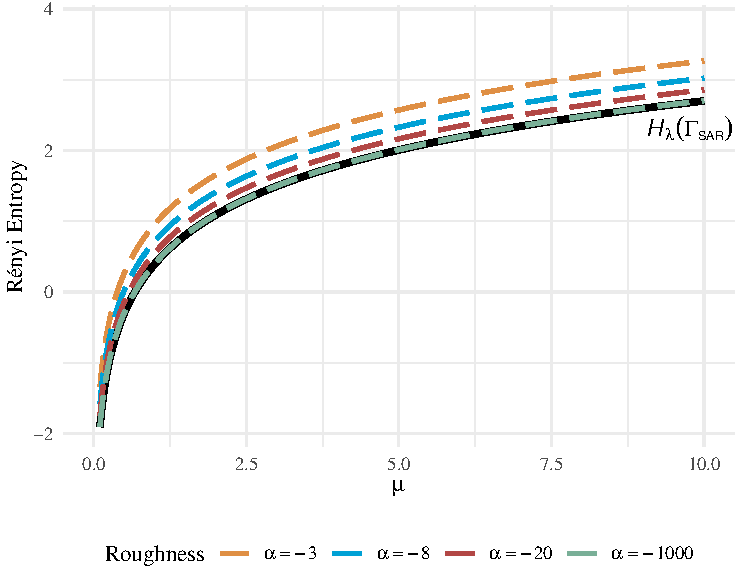
\includegraphics[width=0.45\textwidth,height=\textheight]{Chapters/Chapter2_files/figure-pdf/fig-plot-1.pdf}

}

\end{figure}%

For \(\lambda \to 1\), this expression converges to the Shannon entropy.
As we will see later, this property can lead to improved performance for
heterogeneity detection compared to Shannon entropy.

\section{Main Section 1}\label{main-section-1}

Lorem ipsum dolor sit amet, consectetur adipiscing elit. Aliquam
ultricies lacinia euismod. Nam tempus risus in dolor rhoncus in interdum
enim tincidunt. Donec vel nunc neque. In condimentum ullamcorper quam
non consequat. Fusce sagittis tempor feugiat. Fusce magna erat, molestie
eu convallis ut, tempus sed arcu. Quisque molestie, ante a tincidunt
ullamcorper, sapien enim dignissim lacus, in semper nibh erat lobortis
purus. Integer dapibus ligula ac risus convallis pellentesque.

Let \(\bm{Z}\)

\begin{equation}\phantomsection\label{eq-pmb}{
\int_{A_i}{\lambda (\pmb{\mu})}
}\end{equation}

\begin{equation}\phantomsection\label{eq-mathbf}{
\int_{A_i}{\lambda (\mathbf{x})} + x
}\end{equation}

\subsection{Subsection 1}\label{subsection-1}

Nunc posuere quam at lectus tristique eu ultrices augue venenatis.
Vestibulum ante ipsum primis in faucibus orci luctus et ultrices posuere
cubilia Curae; Aliquam erat volutpat. Vivamus sodales tortor eget quam
adipiscing in vulputate ante ullamcorper. Sed eros ante, lacinia et
sollicitudin et, aliquam sit amet augue. In hac habitasse platea
dictumst.

\begin{figure}[H]

\caption{primera grafica}

{\centering 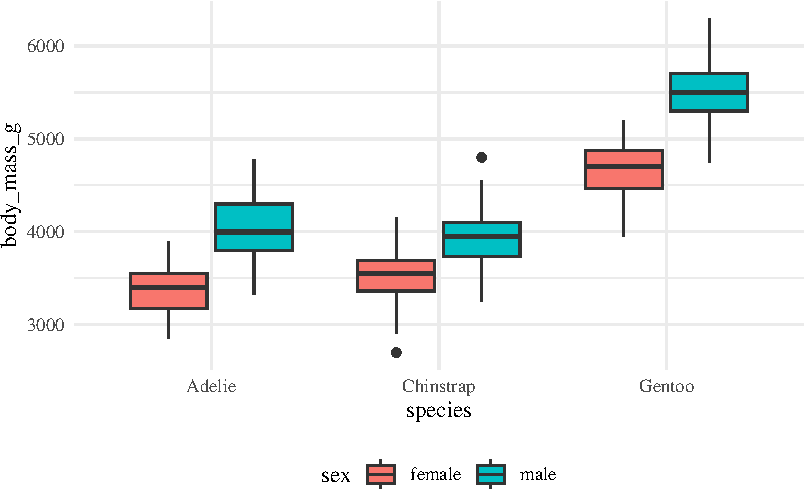
\includegraphics[width=12cm,height=\textheight]{Chapters/Chapter2_files/figure-pdf/unnamed-chunk-2-1.pdf}

}

\end{figure}%

El peso es\textgreater{} 4201.75

\begin{figure}

\caption{\label{fig-charts}Charts}

\begin{minipage}{0.50\linewidth}

\subcaption{\label{fig-charts-1}Cars}

\centering{

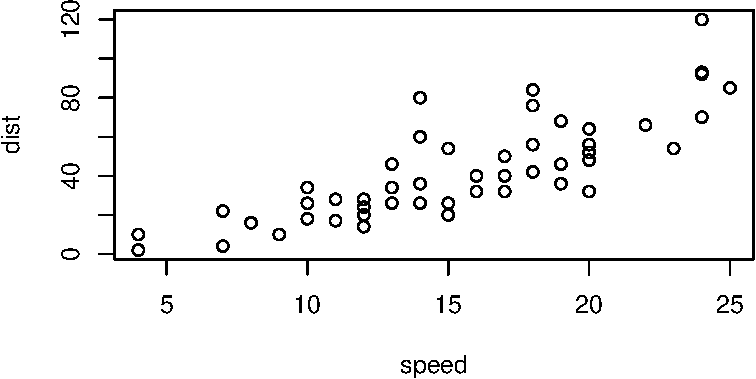
\includegraphics{Chapters/Chapter2_files/figure-pdf/fig-charts-1.pdf}

}

\end{minipage}%
%
\begin{minipage}{0.50\linewidth}

\subcaption{\label{fig-charts-2}Pressure}

\centering{

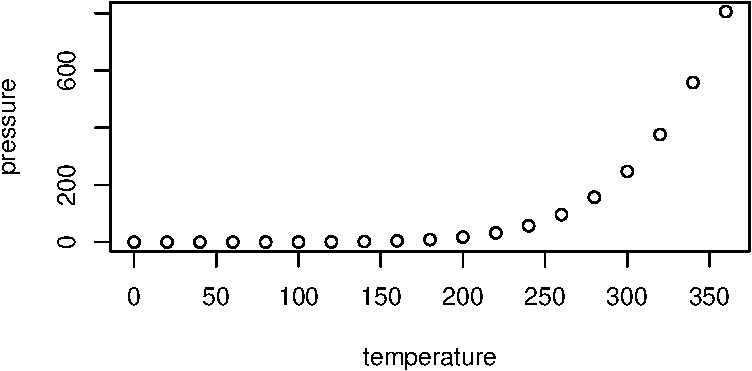
\includegraphics{Chapters/Chapter2_files/figure-pdf/fig-charts-2.pdf}

}

\end{minipage}%

\end{figure}%

\bookmarksetup{startatroot}

\chapter{Tablas}\label{tablas}

\begin{longtable}[]{@{}lll@{}}
\caption{MI primera tabla}\tabularnewline
\toprule\noalign{}
Nombre & \textbf{Apellido} & \textbf{\emph{Telefono}} \\
\midrule\noalign{}
\endfirsthead
\toprule\noalign{}
Nombre & \textbf{Apellido} & \textbf{\emph{Telefono}} \\
\midrule\noalign{}
\endhead
\bottomrule\noalign{}
\endlastfoot
Maria & ss & 45 \\
rosa & sss & 67 \\
\end{longtable}

\begin{longtable}[]{@{}llr@{}}

\caption{\label{tbl-ping}tabla1}

\tabularnewline

\toprule\noalign{}
Especie & sexo & peso \\
\midrule\noalign{}
\endhead
\bottomrule\noalign{}
\endlastfoot
Adelie & female & 3368.836 \\
Adelie & male & 4043.493 \\
Chinstrap & female & 3527.206 \\
Chinstrap & male & 3938.971 \\
Gentoo & female & 4679.741 \\
Gentoo & male & 5484.836 \\

\end{longtable}

Como se muetsra en la tabla Table~\ref{tbl-ping}.

\begin{longtable}[]{@{}ll@{}}
\caption{nueva tabla}\tabularnewline
\toprule\noalign{}
nombre & apellido \\
\midrule\noalign{}
\endfirsthead
\toprule\noalign{}
nombre & apellido \\
\midrule\noalign{}
\endhead
\bottomrule\noalign{}
\endlastfoot
diana & Alpala \\
rosa & Alpala \\
\end{longtable}

\begin{table}
\centering
\caption{Mi tabla}
\centering
\begin{tabular}[t]{rlr}
\toprule
Id & Name & Score\\
\midrule
1 & Alice & 90\\
2 & Bob & 85\\
3 & Charlie & 88\\
4 & Diana & 92\\
5 & Ethan & 80\\
\bottomrule
\end{tabular}
\end{table}

\begin{table}
\centering\centering
\caption{\label{tab:table_param}Parameters of selected SAR images.}
\centering
\resizebox{\ifdim\width>\linewidth\linewidth\else\width\fi}{!}{
\fontsize{12}{14}\selectfont
\begin{tabu} to \linewidth {>{\centering\arraybackslash}p{3.5cm}>{\centering\arraybackslash}p{3cm}>{\centering\arraybackslash}p{2cm}>{\centering\arraybackslash}p{1cm}>{\centering\arraybackslash}p{2cm}>{\centering\arraybackslash}p{2.5cm}>{\centering\arraybackslash}p{1cm}>{\centering\arraybackslash}p{3cm}>{\centering\arraybackslash}p{3cm}}
\toprule
\multicolumn{1}{c}{\textbf{Site}} & \multicolumn{1}{c}{Mission} & \multicolumn{1}{c}{Mode} & \multicolumn{1}{c}{Band} & \multicolumn{1}{c}{Polarization} & \multicolumn{1}{c}{Size} & \multicolumn{1}{c}{$\bm{L}$} & \multicolumn{1}{c}{Resol} & \multicolumn{1}{c}{Date}\\
\midrule
Rotterdam & TerraSAR-X & HS & X & HH & $\bm{512}\times512$ & $1$ & $0.85/0.85$ & 06-12-2018\\
Coast of Jalisco & Sentinel-1B & GRD EW & C & VV & $\textbf{512}    imes512$ & $18$ & $40/40$ & 29-08-2021\\
Illinois-Region 1 & Sentinel-1B & GRD SM & C & VV & $512    imes512$ & $36$ & $10/10$ & 30-06-2020\\
Illinois-Region 2 & Sentinel-1B & GRD SM & C & VV & $1024   imes1024$ & $36$ & $10/10$ & 28-08-2021\\
\bottomrule
\end{tabu}}
\end{table}

\subsection{Subsection 2}\label{subsection-2}

Morbi rutrum odio eget arcu adipiscing sodales. Aenean et purus a est
pulvinar pellentesque. Cras in elit neque, quis varius elit. Phasellus
fringilla, nibh eu tempus venenatis, dolor elit posuere quam, quis
adipiscing urna leo nec orci. Sed nec nulla auctor odio aliquet
consequat. Ut nec nulla in ante ullamcorper aliquam at sed dolor.
Phasellus fermentum magna in augue gravida cursus. Cras sed pretium
lorem. Pellentesque eget ornare odio. Proin accumsan, massa viverra
cursus pharetra, ipsum nisi lobortis velit, a malesuada dolor lorem eu
neque.

\section{Main Section 2}\label{main-section-2}

Sed ullamcorper quam eu nisl interdum at interdum enim egestas. Aliquam
placerat justo sed lectus lobortis ut porta nisl porttitor. Vestibulum
mi dolor, lacinia molestie gravida at, tempus vitae ligula. Donec eget
quam sapien, in viverra eros. Donec pellentesque justo a massa fringilla
non vestibulum metus vestibulum. Vestibulum in orci quis felis tempor
lacinia. Vivamus ornare ultrices facilisis. Ut hendrerit volutpat
vulputate. Morbi condimentum venenatis augue, id porta ipsum vulputate
in. Curabitur luctus tempus justo. Vestibulum risus lectus, adipiscing
nec condimentum quis, condimentum nec nisl. Aliquam dictum sagittis
velit sed iaculis. Morbi tristique augue sit amet nulla pulvinar id
facilisis ligula mollis. Nam elit libero, tincidunt ut aliquam at,
molestie in quam. Aenean rhoncus vehicula hendrerit.

\bookmarksetup{startatroot}

\chapter{PROBLEM STATEMENT AND METHODOLOGY}\label{sec-Chapter3}

\section{Bootstrap Correction for Entropy
Estimators}\label{bootstrap-correction-for-entropy-estimators}

\section{Hypothesis Testing}\label{hypothesis-testing}

\section{Proposed Test Statistics for Heterogeneity
Detection}\label{proposed-test-statistics-for-heterogeneity-detection}

\bookmarksetup{startatroot}

\chapter{CONCLUSIONS AND FUTURE WORK}\label{sec-Chapter5}

\bookmarksetup{startatroot}

\chapter*{REFERENCES}\label{references}
\addcontentsline{toc}{chapter}{REFERENCES}

\markboth{REFERENCES}{REFERENCES}

\phantomsection\label{refs}
\begin{CSLReferences}{0}{1}
\bibitem[\citeproctext]{ref-Frery1997}
FRERY, A. C.; MULLER, H.-J.; YANASSE, C. C. F.; SANTANNA, S. J. S. A
model for extremely heterogeneous clutter. \emph{{IEEE} Transactions on
Geoscience and Remote Sensing}, v. 35, n. 3, p. 648--659, 1997.

\bibitem[\citeproctext]{ref-AlizadehNoughabi2010}
NOUGHABI, A. \href{https://doi.org/10.1080/00949650903005656}{A new
estimator of entropy and its application in testing normality}.
\emph{Journal of Statistical Computation and Simulation}, v. 80, n. 10,
p. 1151--1162, 2010.

\bibitem[\citeproctext]{ref-renyi1961measures}
RÉNYI, A. On measures of entropy and information. 1961, {[}S.l.{]}:
University of California Press, 1961. p. 547--562.

\bibitem[\citeproctext]{ref-Ribeiro2021}
RIBEIRO, M. \emph{et al.} \href{https://doi.org/10.3390/e23020222}{The
Entropy Universe}. \emph{Entropy}, v. 23, n. 2, p. 222, 2021.

\bibitem[\citeproctext]{ref-Shannon1948}
SHANNON, C. E. A Mathematical Theory of Communication. \emph{The Bell
System Technical Journal}, v. 27, n. 3, p. 379--423, 1948.

\bibitem[\citeproctext]{ref-Subhash2021}
SUBHASH, S.; SUNOJ, S. M.; SANKARAN, P. G.; RAJESH, G. Nonparametric
estimation of quantile-based entropy function. \emph{Communications in
Statistics-Simulation and Computation}, v. 52, n. 5, p. 1805--1821,
2021.

\bibitem[\citeproctext]{ref-Wieczorkowski1999}
WIECZORKOWSKI, R.; GRZEGORZEWSKI, P. Entropy estimators-improvements and
comparisons. \emph{Communications in Statistics-Simulation and
Computation}, v. 28, n. 2, p. 541--567, 1999.

\bibitem[\citeproctext]{ref-Zamanzade2012}
ZAMANZADE, E.; ARGHAMI, N. R. Testing normality based on new entropy
estimators. \emph{Journal of Statistical Computation and Simulation}, v.
82, n. 11, p. 1701--1713, 2012.

\end{CSLReferences}

\cleardoublepage
\phantomsection
\addcontentsline{toc}{part}{APPENDICES}
\appendix

\chapter{\texorpdfstring{Derivation of the Rényi Entropy for the
\(\Gamma_{\text{SAR}}(L, \mu)\)
Distribution.}{Derivation of the Rényi Entropy for the \textbackslash Gamma\_\{\textbackslash text\{SAR\}\}(L, \textbackslash mu) Distribution.}}\label{derivation-of-the-ruxe9nyi-entropy-for-the-gamma_textsarl-mu-distribution.}

The Rényi entropy of order \(\lambda\) for a continuous random variable
\(Z\) with density \(f_Z(z)\) is given by \begin{align}
H_\lambda(Z) 
&= \frac{1}{\,1 - \lambda\,} \,\ln \Bigl( \int_{0}^{\infty} [f_Z(z)]^\lambda \, dz \Bigr),
\quad \lambda > 0, \;\lambda \neq 1.
\label{eq:RenyiDefinition}
\end{align}

Let \(Z \sim \Gamma_{\text{SAR}}(L, \mu)\) with pdf \begin{align*}
f_{\Gamma_{\text{SAR}}}(z; L, \mu)
&= \frac{L^L}{\Gamma(L)\,\mu^L}\,z^{\,L - 1} 
  \exp\Bigl(-\tfrac{L z}{\mu}\Bigr)\mathbbm 1_{\mathbbm R_+}(z).
\end{align*} Define \begin{align*}
I 
&= \int_{0}^{\infty}\!\bigl[f_{\Gamma_{\text{SAR}}}(z; L,\mu)\bigr]^\lambda \,dz 
 = \biggl(\frac{L^L}{\Gamma(L)\,\mu^L}\biggr)^{\!\lambda}
   \int_{0}^{\infty} 
   z^{\,\lambda\,(L-1)} \exp\Bigl(-\tfrac{\lambda\,L}{\mu}\,z\Bigr)\,dz.
\end{align*} Using the Gamma integral \(\displaystyle
  \int_{0}^{\infty} x^{p-1} e^{-qx}\,dx
   = \frac{\Gamma(p)}{q^p},\) with \(p = \lambda L - \lambda + 1\) and
\(q = \tfrac{\lambda L}{\mu}\), it follows that \begin{align*}
I 
&= \biggl(\frac{L^L}{\Gamma(L)\,\mu^L}\biggr)^{\!\lambda}
   \frac{\Gamma(\lambda L - \lambda + 1)}
        {\Bigl(\tfrac{\lambda\,L}{\mu}\Bigr)^{\lambda L - \lambda + 1}}.
\end{align*} Taking the natural logarithm, \begin{align}
\ln I 
&= \lambda\Bigl(L \ln L - L \ln \mu - \ln \Gamma(L)\Bigr)
   \;+\; \ln\Gamma\!\bigl(\lambda L - \lambda + 1\bigr)
   \;-\; \bigl(\lambda L - \lambda + 1\bigr)\,\Bigl(\ln(\lambda L) - \ln\mu\Bigr).
\label{eq:lnI}
\end{align} By expanding \eqref{eq:lnI} and collecting terms in
\(\ln L\) and \(\ln \mu\), \begin{align}
\ln I 
&= (1 - \lambda)\bigl(\ln \mu - \ln L\bigr)
   \;-\;\lambda\,\ln \Gamma(L)
   \;+\;\ln\Gamma\!\bigl(\lambda(L-1)+1\bigr)
   \;-\;\bigl(\lambda(L-1)+1\bigr)\,\ln \lambda.
\label{eq:lnIsimplified}
\end{align} Substituting \eqref{eq:lnIsimplified} into
\eqref{eq:RenyiDefinition} and simplifying, \begin{multline}
H_\lambda\bigl(\Gamma_{\text{SAR}}(L,\mu)\bigr) 
= \ln \mu - \ln L 
  + \frac{1}{\,1-\lambda\,}
  \Bigl[
    -\lambda\,\ln\Gamma(L)
    + \ln\Gamma\!\bigl(\lambda\,(L-1)+1\bigr)
    - \bigl(\lambda\,(L-1)+1\bigr)\,\ln\lambda
  \Bigr].
\label{eq:RenyiFinal}
\end{multline} This completes the derivation.

\section{\texorpdfstring{Derivation of the Rényi Entropy for the
\texorpdfstring{$\mathcal{G}^0_I$}{G0I}
Distribution}{Derivation of the Rényi Entropy for the  Distribution}}\label{derivation-of-the-ruxe9nyi-entropy-for-the-distribution}

\medskip

\noindent Let \(Z \sim \mathcal{G}^0_I(\alpha, \gamma, L)\) with pdf
\begin{align*}
f_{\mathcal{G}^0_I}(z; \alpha, \gamma, L) 
&= \frac{L^L\,\Gamma(L-\alpha)}{\gamma^{\alpha}\,\Gamma(-\alpha)\,\Gamma(L)}
   \,\frac{z^{\,L-1}}{\bigl(\gamma + L\,z\bigr)^{\,L-\alpha}}\mathbbm 1_{\mathbbm R_+}(z). \label{E:gamma1}
\end{align*} In particular, this parameterization is consistent with
\(\gamma = -\mu(\alpha + 1)\), so the final expression can be rewritten
in terms of \(\mu\).

\medskip

\noindent Define \begin{align*}
I 
&= \int_{0}^{\infty} \bigl[f_{\mathcal{G}^0_I}(z; \alpha, \gamma, L)\bigr]^\lambda \,dz
= C^\lambda 
  \int_{0}^{\infty} 
    \frac{z^{\,\lambda(L - 1)}}
         {\bigl(\gamma + L\,z\bigr)^{\,\lambda(L - \alpha)}} 
  \,dz,
\end{align*} where \[
C 
= \frac{L^L\,\Gamma(L - \alpha)}{\gamma^\alpha\,\Gamma(-\alpha)\,\Gamma(L)}.
\] Using the change of variables \(t = \tfrac{Lz}{\gamma}\),
\(z = \tfrac{\gamma\,t}{L}\), and \(dz = \tfrac{\gamma}{L}\,dt\), we
obtain \begin{align*}
I 
&= C^\lambda
   \int_{0}^{\infty}
     \Bigl(\tfrac{\gamma\,t}{L}\Bigr)^{\,\lambda(L - 1)}
     \Bigl(\gamma + L\,\tfrac{\gamma\,t}{L}\Bigr)^{-\lambda(L - \alpha)}
     \,\tfrac{\gamma}{L}\,dt
\\
&= C^\lambda 
   \,\frac{\gamma^{\,1+\lambda(\alpha - 1)}}{L^{\,1+\lambda(L - 1)}}
   \int_{0}^{\infty}
     \frac{t^{\,\lambda(L - 1)}}
          {(1 + t)^{\,\lambda(L - \alpha)}}
   \,dt.
\end{align*} By the Beta-function identity \[
\int_{0}^{\infty} \frac{t^{\,a - 1}}{(1 + t)^{\,a + b}} \, dt 
= B(a,b),
\] where \[
a = \lambda(L - 1) + 1,
\quad
b = \lambda(-\alpha + 1) - 1,
\] it follows that \begin{align*}
I 
&= C^\lambda \,\frac{\gamma^{\,1+\lambda(\alpha - 1)}}{L^{\,1+\lambda(L - 1)}}
   \,B(a,b).
\end{align*} Next, we note that
\(\gamma^{\,1 + \lambda(\alpha - 1)} = \gamma^{\,1 - \lambda + \lambda\alpha}\)
and \(L^{\,1 + \lambda(L - 1)} = L^{\,\lambda L + 1 - \lambda}.\) Since
\[
C^\lambda 
= \biggl(\tfrac{L^L}{\gamma^\alpha\,\Gamma(-\alpha)\,\Gamma(L)}\,\Gamma(L - \alpha)\biggr)^{\!\lambda}
= L^{\lambda L}\,\gamma^{-\alpha \lambda}
  \Bigl(\tfrac{\Gamma(L - \alpha)}{\Gamma(-\alpha)\,\Gamma(L)}\Bigr)^\lambda,
\] we obtain \begin{align*}
I
&= \gamma^{\,1 - \lambda}\,
   L^{\,\lambda - 1}
   \Bigl(\tfrac{\Gamma(L - \alpha)}{\Gamma(-\alpha)\,\Gamma(L)}\Bigr)^\lambda
   \,B(a,b).
\end{align*}

\medskip

\noindent By \eqref{eq:RenyiDefinition}, the Rényi entropy, is given by:
\begin{align*}
H_\lambda(Z)
&= \frac{1}{\,1 - \lambda\,} \,\ln I.
\end{align*} Hence, \begin{align*}
H_\lambda(Z) 
&= \frac{1}{\,1 - \lambda\,}
  \,\ln\!\Bigl[
    \gamma^{\,1 - \lambda}\,
    L^{\,\lambda - 1}\,
    \Bigl(\tfrac{\Gamma(L - \alpha)}{\Gamma(-\alpha)\,\Gamma(L)}\Bigr)^\lambda
    \,B(a,b)
  \Bigr].
\end{align*} Thus, for \(Z \sim \mathcal{G}^0_I(\alpha, \gamma, L)\),
\begin{align*}
H_\lambda\bigl(\mathcal{G}^0_I(\alpha, \gamma, L)\bigr)
&= \ln\Bigl(\tfrac{\gamma}{\,L}\Bigr)
  + \frac{1}{\,1 - \lambda\,}
    \Bigl[
      \lambda\bigl(\ln \Gamma(L - \alpha) 
            - \ln \Gamma(-\alpha) 
            - \ln \Gamma(L)\bigr)
      + \ln B(a,b)
    \Bigr].
\end{align*} Using the property \[
\ln B(a,b) 
= \ln \Gamma(a) + \ln \Gamma(b) - \ln \Gamma(a + b),
\] where \(a + b = \lambda(L - \alpha)\), we have \begin{multline}
H_\lambda\bigl(\mathcal{G}^0_I( \alpha,\gamma, L)\bigr)
= \ln\Bigl(\tfrac{\gamma}{L}\Bigr)
 + \frac{1}{\,1 - \lambda\,}
   \Bigl[
     \lambda\bigl(\ln \Gamma(L - \alpha) 
            - \ln \Gamma(-\alpha) 
            - \ln \Gamma(L)\bigr)
     + \ln \Gamma(a)
     + \ln \Gamma(b) \\
     - \ln \Gamma\bigl(\lambda(L - \alpha)\bigr)
   \Bigr].
\label{eq:GI0RenyiInGamma}
\end{multline} Finally, noting that \[
\mu = -\tfrac{\gamma}{\alpha + 1}
\quad\Longrightarrow\quad
\gamma = -\mu(\alpha + 1),
\] and substituting \(\gamma\) into \eqref{eq:GI0RenyiInGamma}, we
obtain \begin{multline}
H_\lambda\bigl(\mathcal{G}^0_I( \alpha,\mu, L)\bigr)
= \ln \mu  -  \ln L + \ln(- 1-\alpha)
+ \frac{1}{\,1 - \lambda\,}
  \Bigl[
    \lambda\Bigl(\ln \Gamma(L - \alpha) 
        - \ln \Gamma(-\alpha) 
        - \ln \Gamma(L)\Bigr)\\
    + \ln \Gamma\bigl(\lambda(L - 1) + 1\bigr)
    + \ln \Gamma\bigl(\lambda(-\alpha + 1) - 1\bigr)
    - \ln \Gamma\bigl(\lambda(L - \alpha)\bigr)
  \Bigr],
\label{eq:RenyiGI0Final}
\end{multline} which completes the derivation.

\section{\texorpdfstring{Relation to the
\texorpdfstring{$\Gamma_{\mathrm{SAR}}$}{Gamma SAR}
Distribution}{Relation to the  Distribution}}\label{relation-to-the-distribution}

The Rényi entropy of the \(\mathcal{G}^0_I(\alpha,\mu,L)\) distribution
can be expressed in terms of the Rényi entropy of the
\(\Gamma_{\mathrm{SAR}}(L,\mu)\) distribution, plus additional terms
involving \(\alpha\) and the Gamma function. Specifically, we can write:
\begin{multline}
H_\lambda\bigl(\mathcal{G}^0_I(\alpha,\mu,L)\bigr)
= 
\underbrace{\Bigl[
  \ln\mu -\ln L + \frac{1}{\,1-\lambda\,}\Bigl(
    -\lambda \,\ln\Gamma(L) 
    +\ln\Gamma\bigl(\lambda(L-1)+1\bigr)
    -\bigl(\lambda(L-1)+1\bigr)\ln\lambda
  \Bigr)
\Bigr]}_{\displaystyle H_\lambda\bigl(\Gamma_{\mathrm{SAR}}(L,\mu)\bigr)}
\\[6pt]
+~\ln\bigl(-1-\alpha\bigr)
+~\frac{1}{\,1-\lambda\,} 
 \Bigl[
   \lambda\bigl(\ln\Gamma(L-\alpha) - \ln\Gamma(-\alpha)\bigr)
   \;+\;\ln\Gamma\bigl(\lambda(-\alpha+1)-1\bigr)
   \;-\;\ln\Gamma\bigl(\lambda(L-\alpha)\bigr) \\
   \;+\;\bigl(\lambda(L-1)+1\bigr)\,\ln(\lambda)
 \Bigr].
\label{eq:GI0_in_terms_of_GammaSAR}
\end{multline} From \eqref{eq:GI0_in_terms_of_GammaSAR}, the bracketed
expression on the first line matches
\(H_\lambda\bigl(\Gamma_{\mathrm{SAR}}(L,\mu)\bigr)\), while the
remaining terms account for the parameter \(\alpha\) through additional
Gamma functions and logarithmic corrections. This decomposition
highlights the close relationship between the Rényi entropies of the
\(\mathcal{G}^0_I\) and \(\Gamma_{\mathrm{SAR}}\) distributions.

\chapter{\texorpdfstring{Limit Behavior of
\texorpdfstring{$H_\lambda(\mathcal{G}^0_I)$}{Hl(GI0)} as
\texorpdfstring{$\alpha \to -\infty$}{alpha->-∞}}{Limit Behavior of  as }}\label{limit-behavior-of-as}

We want to show that \[
\lim_{\alpha \to -\infty}
H_\lambda\bigl(\mathcal{G}^0_I\bigr)(\mu, \alpha, L)
=
H_\lambda\bigl(\Gamma_{\mathrm{SAR}}\bigr)(\mu, L).
\]

We can express \eqref{eq:GI0_in_terms_of_GammaSAR} as follows:
\begin{align*}
H_\lambda\bigl(\mathcal{G}^0_I\bigr)(\mu,\alpha,L)
&=
H_\lambda\bigl(\Gamma_{\mathrm{SAR}}\bigr)(\mu,L)
\;+\;
\ln\!\bigl(-1-\alpha\bigr)
\\
&\quad
+ \frac{1}{1-\lambda}
\ln \Biggl[
  \frac{
    \Gamma(L-\alpha)^{\lambda}\,\Gamma\bigl(\lambda(-\alpha+1)-1\bigr)\,\lambda^{\lambda(L-1)+1}
  }{
    \Gamma(-\alpha)^{\lambda}\,\Gamma\bigl(\lambda(L-\alpha)\bigr)
  }
\Biggr].
\end{align*} Set \begin{align*}
\Delta(\alpha)
&=
H_\lambda\bigl(\mathcal{G}^0_I\bigr)(\mu,\alpha,L)
-
H_\lambda\bigl(\Gamma_{\mathrm{SAR}}\bigr)(\mu,L).
\end{align*} Then \begin{align}
\Delta(\alpha)
=
\ln(-1-\alpha)
+
\frac{1}{1-\lambda}
\ln \biggl[
  \frac{
    \Gamma(L-\alpha)^{\lambda}\,\Gamma\bigl(\lambda(-\alpha+1)-1\bigr)\,\lambda^{\lambda(L-1)+1}
  }{
    \Gamma(-\alpha)^{\lambda}\,\Gamma\bigl(\lambda(L-\alpha)\bigr)
  }
\biggr].
\label{eq:remain}
\end{align}

As \(\alpha \to -\infty\), we have \(-1-\alpha \approx |\alpha|\), so \[
\ln(-1-\alpha) 
\sim 
\ln|\alpha|.
\] Note that for large \(|\alpha|\), we can the asymptotic relation
\(\Gamma(x+a)/\Gamma(x+b)\sim x^{\,a-b}\). Specifically: \[
\Gamma(L-\alpha)/\Gamma(-\alpha) \;\sim\; |\alpha|^L,
\quad
\Gamma\bigl(\lambda(-\alpha+1)-1\bigr)/\Gamma\bigl(\lambda(L-\alpha)\bigr)
\;\sim\; 
\bigl(\lambda|\alpha|\bigr)^{\,(\lambda-1)-\lambda L}.
\] Thus, inside the logarithm in \eqref{eq:remain}, \[
\frac{
  \Gamma(L-\alpha)^{\lambda}\,\Gamma\bigl(\lambda(-\alpha+1)-1\bigr)
}{
  \Gamma(-\alpha)^{\lambda}\,\Gamma\bigl(\lambda(L-\alpha)\bigr)
}
\;\sim\;
|\alpha|^{\lambda L}
\times
|\alpha|^{(\lambda-1)-\lambda L}
=
|\alpha|^{\,\lambda-1}.
\] Since \(\lambda^{\lambda(L-1)+1}\) does not depend on \(\alpha\),
multiplying by this constant factor does not alter the asymptotic
behavior in \(\alpha\). Therefore, \[
\frac{1}{1-\lambda}\,
\ln\!\Bigl[\dots\Bigr]
\;\sim\;
\frac{1}{1-\lambda}\;\ln\!\bigl(|\alpha|^{\,\lambda-1}\bigr)
=
\frac{\lambda-1}{1-\lambda}\,\ln|\alpha|
=
-\ln|\alpha|.
\] Hence \[
\Delta(\alpha)
\;\sim\;
\ln|\alpha|
-
\ln|\alpha|
=
0
\quad
\text{as}\, \alpha\to -\infty.
\] This shows \(\Delta(\alpha)\to 0\), and consequently \[
\lim_{\alpha \to -\infty}
H_\lambda\bigl(\mathcal{G}^0_I\bigr)(\mu,\alpha,L)
=
H_\lambda\bigl(\Gamma_{\mathrm{SAR}}\bigr)(\mu,L).
\]



\end{document}
